\documentclass[12pt]{article}
\usepackage{setspace}
\usepackage{natbib}
\usepackage{graphicx}
\usepackage{xcolor}
\usepackage[scaled]{helvet}
\usepackage[T1]{fontenc}
\usepackage[margin=1in]{geometry}
\usepackage[fleqn]{amsmath}
\usepackage{amssymb}
\usepackage{bm}
\usepackage{subcaption}
\usepackage{listings}
\usepackage{float}
\usepackage{tikz}
\usepackage{fancyhdr}
\lstset{language=Python,
    frame=single,
    breaklines=true,
    postbreak=\raisebox{0ex}[0ex][0ex]{\ensuremath{\color{red}\hookrightarrow\space}}
}

\restylefloat{figure}
\newcommand{\Prop}{\textbf{Proposition: }}
\newcommand{\Prob}{\textbf{Problem: }}
\newcommand{\Prf}{\textbf{Proof: }}
\newcommand{\Sol}{\textbf{Solution: }}
\newcommand{\grad}{\nabla}
\newcommand{\Nats}{\mathbb{N}}
\newcommand{\Ints}{\mathbb{Z}}
\newcommand{\Rats}{\mathbb{Q}}
\newcommand{\Reals}{\mathbb{R}}
\newcommand{\Comps}{\mathbb{C}}
\newcommand{\Prb}[1]{P\left( #1 \right)}
\newcommand{\PT}[1]{P\left( \text{#1} \right)}
\newcommand{\PCon}[2]{P\left( #1 \mid #2 \right)}
\newcommand{\PConT}[2]{P\left( \text{#1} \mid \text{#2} \right)}
\DeclareMathOperator{\E}{\mathbb{E}}
\DeclareMathOperator{\tr}{\textbf{tr}}
\DeclareMathOperator*{\argmin}{argmin}
\DeclareMathOperator*{\argmax}{argmax}
\newcommand{\thus}{\quad\mathlarger{\mathlarger{\mathlarger{\Rightarrow}}}\quad}
\newcommand{\wght}{\mathbf{w}}
\newcommand{\im}{\text{im }}
%%\newcommand\scalemath[2]{\scalebox{#1}{\mbox{\ensuremath{\displaystyle #2}}}}


%% Tikz stuff
\usetikzlibrary{shapes,arrows}
\usetikzlibrary{decorations.pathreplacing, decorations.pathmorphing, snakes, calligraphy}

\tikzstyle{block} = [rectangle, draw, thick, align=center, rounded corners]
\tikzstyle{boundingbox} = [very thick, gray]
\tikzstyle{dashblock} = [rectangle, draw, thick, align=center, dashed]
\tikzstyle{conc} = [ellipse, draw, thick, dashed, align=center]
\tikzstyle{netnode} = [circle, draw, very thick, inner sep=0pt, minimum size=0.5cm]
\tikzstyle{relunode} = [rectangle, draw, very thick, inner sep=0pt, minimum size=0.5cm]
\tikzstyle{line} = [draw, very thick, -latex']
\tikzstyle{arrow} = [draw, ->, thick]
\tikzstyle{mapsto} = [draw, |->, thick]

\def\checkmark{\tikz\fill[scale=0.4](0,.35) -- (.25,0) -- (1,.7) -- (.25,.15) -- cycle;}


%% Some colors stolen from ColorBrewer
\definecolor{bpurp}{HTML}{984ea3}
\definecolor{bblue}{HTML}{377eb8}
\definecolor{bgreen}{HTML}{4daf4a}
\definecolor{borange}{HTML}{ff7f00}
\definecolor{bred}{HTML}{a50f15}

% footnote without a marker
\makeatletter
\def\blfootnote{\gdef\@thefnmark{}\@footnotetext}
\makeatother



\renewcommand{\headrulewidth}{0pt}
\renewcommand{\footrulewidth}{0.4pt}


\pagestyle{fancy}
\fancyhf{}
\rhead{Andrew K. Lampinen}
\rfoot{\thepage}

\fancypagestyle{firststyle}
{
  \fancyhf{}
  \rfoot{\thepage}
}

\def\bigcheckmark{\tikz\fill[scale=0.66](0,.35) -- (.25,0) -- (1,.7) -- (.25,.15) -- cycle;}

\doublespacing

\renewcommand\familydefault{\sfdefault}
\title{A computational framework for learning and transforming task representations}
\author{Andrew Kyle Lampinen}
\date{}
\begin{document}
\maketitle
\thispagestyle{firststyle}

Humans exhibit substantial cognitive flexibility. We can use our knowledge of a task to adapt to novel variations on our first try. For example, imagine you are playing poker with your friends, and one of them says ``next round, let's try to lose.'' You will be able to perform well, despite the new goal directly contradicting your prior goal. Alternatively, suppose your friend says ``next round, threes will be wild.'' You will be able to play this variation, even if you have never played it before. For an example from another domain, imagine your friend shows you a blue car, and then tells you that their car looks similar, except that it is red. You will be able to combine these pieces of knowledge to recognize their car, despite never having seen it before. Humans can adapt our knowledge to a new situation on our first try. 

By contrast, while deep learning models can achieve human (or super-human) performance at games \citep{Silver2017,Vinyals2019} and object recognition \citep{Szegedy2016}, they are unable to flexibly adapt their knowledge of these tasks \citep{Lake2016}. How could a deep learning model trained to win at poker reuse that knowledge to try to lose? How could a model trained to recognize one car adapt to recognize that car in a different color? Many deep learning models cannot, even in principle.  

Observations like these have formed a key piece of contemporary critiques of deep learning models as cognitive models \citep{Lake2016,Marcus2018}. These critiques echo criticisms of the generalization capabilities of neural networks from the earlier days of connectionism \citep{Fodor1988}. Can deep learning serve as a foundation for plausible cognitive models, or is the approach fundamentally limited, as these critiques suggest? 

In this dissertation, I bring new light to this debate, by proposing and demonstrating a novel approach to adaptation in deep learning models. The method is based on interpreting the types of adaptation above as transformations of tasks. For example, there might be a ``try-to-lose'' transformation that would transform poker to a losing variation of poker, chess to a losing variation of chess, etc. I therefore propose a general framework for both learning task representations, and learning to transform those task representations in order to adapt to new tasks. This learning-based approach does not require building in prior knowledge about the structure of the tasks, or compositional symbolic reasoning. Instead, the transformations are learned solely from relationships between learned representations of tasks. 
\renewcommand{\headrulewidth}{0.4pt}

My approach allows deep learning models to flexibly reuse their knowledge of a task to adapt to novel variations of that task. In fact, my approach demonstrates 80-90\% performance on novel tasks across a broad range of domains, including simple card games and video games, and visual classification. Furthermore, this adaptation allows the model to learn the novel tasks much more efficiently. This shows that deep learning models can flexibly reuse their knowledge to perform well on their first try, and learn rapidly, without requiring built-in prior domain knowledge, or symbolic reasoning systems. 

This work therefore has broad implications. It addresses fundamental questions about the computational approaches necessary for flexible intelligence, and how that flexibility can contribute to later learning. This has implications for cognitive science, neuroscience, and philosophy of mind. In addition, I demonstrate the approach within several important contemporary artificial intelligence paradigms, including visual classification and deep reinforcement learning. It may therefore also be of interest to researchers who wish to build more flexible artificial intelligence and machine learning systems.

\section{The method: adaptation as task transformation}

My approach is based on the idea that tasks can be seen as mappings from inputs to outputs. For example, poker can be seen as a mapping of hands to bets (Fig. \ref{fig:HoMM:tasks_as_mappings:basic}), and visual classification can be seen as a mapping from images to classifications. I suggest that to perform many of these tasks flexibly, as humans can, we must be able to constrain these mappings by an internal representation of the current task. I therefore draw inspiration from both cognitive science and machine learning, and allow my model to construct a task representation from either a language cue, or examples of the task (Fig. \ref{fig:HoMM_architecture:constructing_basic}). 

The model then uses its internal representation of the current task to adapt to that task (Fig. \ref{fig:HoMM_architecture:performing_basic}). Specifically, the task representation sets the weights of a task network to make appropriate decisions, for example to respond positively to straight flushes when playing poker. 

The key insight of my dissertation is that the task representations that the model has constructed can then be transformed to adapt to new tasks. By transforming a prior task representation, the model can perform a new task without having experienced it, just as humans can adapt to new tasks by transforming their prior knowledge. Specifically, I allow the model to construct a representation of a task transformation from a language cue (``try to lose'') or examples of the transformation (trying to win and lose at various other games), see Fig. \ref{fig:HoMM_architecture:constructing_meta}. This representation of the transformation can then be used to adapt to that transformation, by setting the weights of a task network to appropriately transform task representations (Fig. \ref{fig:HoMM_architecture:performing_meta}). For example, the system could apply the ``try-to-lose'' transformation to its representation of poker to produce a representation of the task of losing at poker. This representation could then be used to perform that task (Fig \ref{fig:HoMM_architecture:performing_meta}-detail). 

There is an analogy between the basic tasks and meta-mappings --- both are simply functions from inputs to outputs, just of different types. The implementation I propose, called the HoMM architecture, therefore parsimoniously reuses the same architectural components for both basic tasks and transformations of basic tasks. This parallel is reflected in the parallels between the top and bottom rows of Fig. \ref{fig:HoMM_architecture}. This approach is parsimonious, in that it does not multiply networks unnecessarily. It also reflects ideas from the theory of programming languages, and aspects of the Global Workspace Theory of consciousness \citep{Baars2005}. 


\begin{figure}[h]
\singlespacing
\centering
\begin{subfigure}{0.4\textwidth}
\centering
\begin{tikzpicture}[auto]
%% a) basic task
\draw[boundingbox, draw=gray, fill=white] (-2.75, -2.5) rectangle (2.75, 2.5);
\node[gray, text width=2cm, align=center] at (0, 2.1) {Poker task};
\begin{scope}[shift={(0,-0.5)}]
\node[text width=0.5cm] at (-1.5, -1.3) {\includegraphics[width=0.5cm]{2-HoMM/figures/4_of_hearts.png}};
\node[text width=0.5cm] at (-1.35, -1.25) (pokerin0) {\includegraphics[width=0.5cm]{2-HoMM/figures/2_of_spades.png}};
\node[text width=0.5cm] at (1.35, -1.25) (pokerout0) {\bf ?};
\path[mapsto] (pokerin0) to (pokerout0);
\end{scope}
\begin{scope}[shift={(0,0.5)}]
\node[text width=0.5cm] at (-1.5, -1.3) {\includegraphics[width=0.5cm]{2-HoMM/figures/3_of_spades.png}};
\node[text width=0.5cm] at (-1.35, -1.25) (pokerin0) {\includegraphics[width=0.5cm]{2-HoMM/figures/4_of_hearts.png}};
\node[text width=0.5cm] at (1.35, -1.25) (pokerout0) {\bf \$1};
\path[mapsto] (pokerin0) to (pokerout0);
\end{scope}
\begin{scope}[shift={(0,1.5)}]
\node[text width=0.5cm] at (-1.5, -1.3) {\includegraphics[width=0.5cm]{2-HoMM/figures/ace_of_spades.png}};
\node[text width=0.5cm] at (-1.35, -1.25) (pokerin0) {\includegraphics[width=0.5cm]{2-HoMM/figures/2_of_spades.png}};
\node[text width=0.5cm] at (1.35, -1.25) (pokerout0) {\bf \$2};
\path[mapsto] (pokerin0) to (pokerout0);
\end{scope}
\begin{scope}[shift={(0,2.5)}]
\node[text width=0.5cm] at (-1.5, -1.3) {\includegraphics[width=0.5cm]{2-HoMM/figures/4_of_hearts.png}};
\node[text width=0.5cm] at (-1.35, -1.25) (pokerin0) {\includegraphics[width=0.5cm]{2-HoMM/figures/ace_of_spades.png}};
\node[text width=0.5cm] at (1.35, -1.25) (pokerout0) {\bf \$0};
\path[mapsto] (pokerin0) to (pokerout0);
\end{scope}

\end{tikzpicture}
\caption{A basic task.} \label{fig:HoMM:tasks_as_mappings:basic}
\end{subfigure}
\begin{subfigure}{0.4\textwidth}
\centering
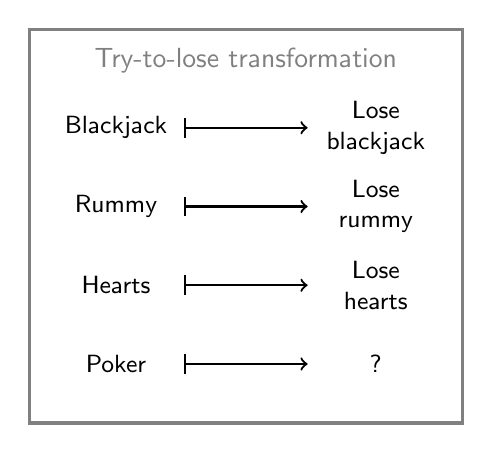
\begin{tikzpicture}[auto]
\small
\draw[boundingbox, draw=gray, fill=white] (-2.75, -2.5) rectangle (2.75, 2.5);

\node[gray, align=center] at (0, 2.1) {\normalsize Try-to-lose transformation};
\begin{scope}[shift={(0,-0.5)}]
\node[text width=1.5cm, align=center] at (-1.65, -1.25) (metain0) {Poker};
\node[text width=1.5cm, align=center] at (1.65, -1.25) (metaout0) {?};
\path[mapsto] (metain0) to (metaout0);
\end{scope}

\begin{scope}[shift={(0,0.5)}]
\node[text width=1.5cm, align=center] at (-1.65, -1.25) (metain0) {Hearts};
\node[text width=1.5cm, align=center] at (1.65, -1.25) (metaout0) {Lose hearts};
\path[mapsto] (metain0) to (metaout0);
\end{scope}

\begin{scope}[shift={(0,1.5)}]
\node[text width=1.5cm, align=center] at (-1.65, -1.25) (metain0) {Rummy};
\node[text width=1.5cm, align=center] at (1.65, -1.25) (metaout0) {Lose rummy};
\path[mapsto] (metain0) to (metaout0);
\end{scope}

\begin{scope}[shift={(0,2.5)}]
\node[text width=1.5cm, align=center] at (-1.65, -1.25) (metain0) {Blackjack};
\node[text width=1.5cm, align=center] at (1.65, -1.25) (metaout0) {Lose blackjack};
\path[mapsto] (metain0) to (metaout0);
\end{scope}
\end{tikzpicture}
\caption{A task transformation.} \label{fig:HoMM:tasks_as_mappings:meta}
\end{subfigure}
\caption[Basic tasks and meta-mappings.]{Basic tasks and task transformations. (\subref{fig:HoMM:tasks_as_mappings:basic}) Basic tasks can be seen as mappings from inputs to outputs, for example, from poker hands to bets. Tasks can be generalized from examples. (\subref{fig:HoMM:tasks_as_mappings:meta}) Task transformations are higher-order tasks, which take a basic task as input, and output a transformed version of that task, for example, switching from winning to losing a game. Task transformations can be generalized from examples.} \label{fig:HoMM:tasks_as_mappings}
\end{figure}

\begin{figure}[htbp]
\centering
\singlespacing
\resizebox{\textwidth}{!}{%
\begin{tikzpicture}[auto]

\begin{scope}[shift={(0.4,0)}]
%% b) constructing
\draw[boundingbox, draw=gray, fill=white] (-8.5, -2.5) rectangle (-2, 2.6);

%% from language
\node[gray] at (-7, 2.1) {\small Instructions};
\node at (-7, 1.25) (language) {``Play poker.''};

\node[gray, text width=2cm, align=center] at (-4.1, 2.1) {\small Language network};
\node[block] at (-4.1, 1.25) (languagenet) {\(\mathcal{L}\)}; 
\path[arrow] (language.east) -- ([xshift=-3]languagenet.west);

\node[bpurp, text width=2cm] at (-2, 1.25) (languagetaskrep) {\(z_{task}\)}; 
\path[arrow] ([xshift=3]languagenet.east) -- (languagetaskrep.west);


%% from examples

\node[gray, text width=2.5cm, align=center] at (-7, -0.1) {\small Task examples (encoded)};
\node at (-7, -1.25) (examples) {
\(\left\{
\begin{matrix}
({\color{bgreen}z_{hand_{1}}}, {\color{bgreen}z_{bet_{1}}})\\
$\vdots$
\end{matrix}\right\}\)};

\node[gray, text width=2cm, align=center] at (-4.1, -0.4) {\small Example network};
\node[block] at (-4.1, -1.25) (examplenet) {\(\mathcal{E}\)}; 
\path[arrow] (examples.east) -- ([xshift=-3]examplenet.west);

\node[bpurp, text width=2cm] at (-2, -1.25) (examplestaskrep) {\(z_{task}\)}; 
\path[arrow] ([xshift=3]examplenet.east) -- (examplestaskrep.west);

\end{scope}

%% c) performing 
\draw[boundingbox, draw=gray, fill=white] (-1.5, -2.5) rectangle (8.5, 2.6);
\node[bpurp] at (-0.75, 1.25) (taskrep) {\(z_{task}\)};

\node[gray, text width=2cm, align=center] at (0.75, 2.1) {\small Hyper network};
\node[block] at (0.75, 1.25) (hypernet) {\(\mathcal{H}\)}; 
\path[arrow] (taskrep.east) -- ([xshift=-3]hypernet.west);

\node[text width=0.5cm] at (-1, -1.3) {\includegraphics[width=0.5cm]{2-HoMM/figures/4_of_hearts.png}};
\node[text width=0.5cm] at (-0.85, -1.25) (inputs) {\includegraphics[width=0.5cm]{2-HoMM/figures/2_of_spades.png}};

\node[gray, text width=2cm, align=center] at (0.6, -2) {\small Perception network};
\node[block] at (0.6, -1.25) (perceptionnet) {\(\mathcal{P}\)}; 
\path[arrow] (inputs.east) -- ([xshift=-3]perceptionnet.west);

\node[bgreen] at (2.05, -1.25) (handrep) {\(z_{hand}\)};
\path[arrow] ([xshift=3]perceptionnet.east) -- (handrep.west);

\node[bblue, block, dashed] at (3.5, -1.25) (tasknet) {\(\mathcal{T}\)}; 
\node[bblue, text width=1.5cm, align=center] at (3.5, -2) {\small Task network};
\path[arrow] (handrep.east) -- ([xshift=-3]tasknet.west);
\path[arrow, out=0, in=90] ([xshift=3]hypernet.east) to ([yshift=3]tasknet.north);


\node[bgreen] at (4.85, -1.25) (betrep) {\(z_{bet}\)};
\path[arrow] ([xshift=3]tasknet.east) -- (betrep.west);

\node[gray, text width=2cm, align=center] at (6.2, -2) {\small Action network};
\node[block] at (6.2, -1.25) (actionnet) {\(\mathcal{A}\)}; 
\path[arrow] (betrep.east) -- ([xshift=-3]actionnet.west);

\node at (7.4, -1.25) (output) {\bf \$};
\path[arrow] ([xshift=3]actionnet.east) -- (output.west);

%% d subpanel) task network

\draw[boundingbox, draw=gray, fill=white] (4.25, 0) rectangle (8.5, 2.6);
\node[gray] at (6.35, 2.25) {\small \(\mathcal{H}\) adapts all weights in \(\mathcal{T}\)};

\node at (4.45, 1.45) (pseudohyper) {};

\node[bblue] at (5.25, 1.65) (Wprime) {\scriptsize \(W'\), \(b'\) (from \(\mathcal{H}\))};
\node[bblue] at (6.05, 0.25) (W0) {\scriptsize Default \(W^{0}\), \(b^{0}\)};
\node[netnode, bblue, thick] at (4.75, 0.5) (tnode1) {I};

\node[netnode, bblue, thick] at (7.35, 0.5) (tnode2) {O};
\node[bblue] at (7.35, 1.4) {\scriptsize\(O\!=\!(W^{0}\!+\!W') I\)};
\node[bblue] at (7.4, 1.1) {\scriptsize\(+(b^{0}\!+\!b')\)};

\path[arrow, bblue, out=0, in=90] (pseudohyper) to ([yshift=10]W0);
\path[arrow, bblue, dashed] (tnode1) to (tnode2);

%% connecting to subpanel

\path[draw, gray, thick] (3.75, -0.95) to (4.25, 2.5);
\path[draw, gray, thick] (3.75, -0.95) to (8.5, 0);
\end{tikzpicture}
}
\begin{subfigure}[t]{0.39\textwidth}%%Haaaaaacky
\vspace{-1em}
\caption{Constructing a basic-task representation.}\label{fig:HoMM_architecture:constructing_basic}
\vspace{0.5em}
\end{subfigure}%
\begin{subfigure}[t]{0.61\textwidth}
\vspace{-1em}
\caption{Performing a basic task from its representation.}\label{fig:HoMM_architecture:performing_basic}
\vspace{0.5em}
\end{subfigure}
\resizebox{\textwidth}{!}{%
\begin{tikzpicture}[auto]
\begin{scope}[shift={(0.4,0)}]
%% a) constructing
\draw[boundingbox, draw=gray, fill=white] (-8.5, -2.5) rectangle (-2, 2.6);

%% from language
\node[gray] at (-6.7, 2.1) {\small Instructions};
\node at (-6.7, 1.25) (language) {``Try to lose.''};

\node[gray, text width=2cm, align=center] at (-4.1, 2.1) {\small Language network};
\node[block] at (-4.1, 1.25) (languagenet) {\(\mathcal{L}\)}; 
\path[arrow] (language.east) -- ([xshift=-3]languagenet.west);

\node[borange, text width=2cm] at (-2, 1.25) (languagetaskrep) {\(z_{trns}\)}; 
\path[arrow] ([xshift=3]languagenet.east) -- (languagetaskrep.west);


%% from examples

\node[gray, text width=3.5cm, align=center] at (-6.7, -0.1) {\small Mapping examples (input/output tasks)};
\node at (-6.7, -1.25) (examples) {
\(\left\{
\begin{matrix}
\!({\color{bpurp}z_{heart}}, {\color{bpurp}z_{lose heart}})\!\\
$\vdots$
\end{matrix}\right\}\)};

\node[gray, text width=2cm, align=center] at (-4.1, -0.4) {\small Example network};
\node[block] at (-4.1, -1.25) (examplenet) {\(\mathcal{E}\)}; 
\path[arrow] (examples.east) -- ([xshift=-3]examplenet.west);

\node[borange, text width=2cm] at (-2, -1.25) (examplestaskrep) {\(z_{trns}\)}; 
\path[arrow] ([xshift=3]examplenet.east) -- (examplestaskrep.west);
\end{scope}

%% d) performing 
\draw[boundingbox, draw=gray, fill=white] (-1.5, -2.5) rectangle (8.5, 2.6);
\node[borange] at (-0.75, 1.25) (taskrep) {\(z_{trns}\)};

\node[gray, text width=2cm, align=center] at (0.75, 2.1) {\small Hyper network};
\node[block] at (0.75, 1.25) (hypernet) {\(\mathcal{H}\)}; 
\path[arrow] (taskrep.east) -- ([xshift=-3]hypernet.west);

\node[bpurp] at (1.66, -1.25) (handrep) {\(z_{poker}\)};

\node[bblue, block, dashed] at (3.5, -1.25) (tasknet) {\(\mathcal{T}\)}; 
\node[bblue, text width=1.5cm, align=center] at (3.5, -2) {\small Task network};
\path[arrow] (handrep.east) -- ([xshift=-3]tasknet.west);
\path[arrow, out=0, in=90] ([xshift=3]hypernet.east) to ([yshift=3]tasknet.north);

\node[bpurp] at (5.5, -1.25) (output) {\(z_{lose poker}\)};
\path[arrow] ([xshift=3]tasknet.east) -- (output.west);

%% d subpanel) performing basic from meta-mapped

\draw[boundingbox, draw=gray, fill=white] (4.25, 0) rectangle (8.5, 2.6);
\node[gray] at (6.35, 2.25) {\small Performing the new task};
\begin{scope}[scale=0.5, shift={(8.5,2.5)}, every node/.append style={transform shape}]

\node[gray, text width=2cm, align=center] at (2, 1.1) {Hyper network};
\node[block, semithick, rounded corners=2] at (2, 0.25) (hypernet2) {\(\mathcal{H}\)}; 

\node[text width=0.5cm] at (0.55, -1.3) {\includegraphics[width=0.5cm]{2-HoMM/figures/4_of_hearts.png}};
\node[text width=0.5cm] at (0.7, -1.25) (inputs2) {\includegraphics[width=0.5cm]{2-HoMM/figures/2_of_spades.png}};

\node[gray, text width=2cm, align=center] at (1.9, -2) {Perception network};
\node[block, semithick, rounded corners=2] at (1.9, -1.25) (perceptionnet2) {\(\mathcal{P}\)}; 
\path[arrow, semithick] (inputs2.east) -- ([xshift=-3]perceptionnet2.west);

\node[bgreen] at (3.2, -1.25) (handrep2) {\(z_{hand}\)};
\path[arrow, semithick] ([xshift=3]perceptionnet2.east) -- (handrep2.west);

\node[bblue, block, semithick, rounded corners=2, dash pattern=on 2pt off 2pt] at (4.5, -1.25) (tasknet2) {\(\mathcal{T}\)}; 
\node[bblue, text width=1.5cm, align=center] at (4.5, -2) {Task network};
\path[arrow, semithick] (handrep2.east) -- ([xshift=-3]tasknet2.west);
\path[arrow, semithick, out=0, in=90] ([xshift=3]hypernet2.east) to ([yshift=3]tasknet2.north);

\node[bgreen] at (5.65, -1.25) (betrep2) {\(z_{bet}\)};
\path[arrow, semithick] ([xshift=3]tasknet2.east) -- (betrep2.west);

\node[gray, text width=2cm, align=center] at (6.8, -2) {Action network};
\node[block, semithick, rounded corners=2] at (6.8, -1.25) (actionnet2) {\(\mathcal{A}\)}; 
\path[arrow, semithick] (betrep2.east) -- ([xshift=-3]actionnet2.west);

\node at (7.8, -1.25) (output2) {\bf \$};
\path[arrow] ([xshift=3]actionnet2.east) -- (output2.west);
\end{scope}

%% connecting to subpanel

\node[inner sep=0, outer sep=0] at (6.8, -0.8) (c1) {};
\node[inner sep=0, outer sep=0] at (4.5, -0.3) (c2) {};
\node[inner sep=0, outer sep=0] at (4, 0.5) (c3) {};
\path[draw, gray, very thick, out=0, in=-90, dash pattern=on 2pt off 2pt] (output.east) to (c1);
\path[draw, gray, very thick, out=90, in=0, dash pattern=on 2pt off 2pt] (c1) to (c2);
\path[draw, gray, very thick, out=180, in=-90, dash pattern=on 2pt off 2pt] (c2) to (c3);
\path[arrow, gray, very thick, out=90, in=180, dash pattern=on 2pt off 2pt] (c3) to ([xshift=-3]hypernet2.west);

\end{tikzpicture}
}
\begin{subfigure}[t]{0.4\textwidth}
\vspace{-1em}
\caption{Constructing a task-\phantom{blahblahblahblah}  transformation representation.}\label{fig:HoMM_architecture:constructing_meta}
\end{subfigure}%
\begin{subfigure}[t]{0.6\textwidth}
\vspace{-1em}
\caption{Transforming a basic task representation, by using a representation of the task transformation.}\label{fig:HoMM_architecture:performing_meta}
\end{subfigure}
\caption[Performing and transforming tasks with the HoMM architecture.]{A homogeneous architecture for performing and transforming tasks. (\subref{fig:HoMM_architecture:constructing_basic},\subref{fig:HoMM_architecture:constructing_meta}) The HoMM architecture performs basic tasks and task transformations from a task representation, which can be constructed from appropriate language inputs or examples.  (\subref{fig:HoMM_architecture:performing_basic}) The task representation is used to alter the parameters of a task network (see detail) which executes the appropriate task mapping. (\subref{fig:HoMM_architecture:performing_meta}) The task transformation representation is used to parameterize the task network to transform a task representation. The transformed representation can then be used to perform the new task without any direct experience of the new task (see detail). The HoMM architecture exploits a deep analogy between basic tasks and task transformations --- both can be seen as mappings of inputs to outputs, although they have different types of inputs and outputs. Thus, the architecture uses type-specific models to embed all basic inputs, as well as tasks and task transformations, in a shared representational space. Then all tasks and task transformations can be seen as transformations applied to entities in this space, which can be executed by shared systems. The parallels between the basic tasks and the task transformations are reflected in the parallels between the top and bottom rows of the figure.} \label{fig:HoMM_architecture}
\end{figure}



\section{Selected experimental results}
\textbf{Card games:} I demonstrate my approach in a domain of simple card games. I show that my architecture is able to learn to play card games nearly optimally, and from seeing examples on other games, it is able to transform its representation of simplified poker to play a novel losing variation of that game on its first try, and achieve 85\% of optimal performance on this difficult adaptation. This is achieved without giving the system prior knowledge of winning, losing, or any of the concepts relevant to the games, based only on performing tasks and seeing the relationship between winning and losing at other games.

I compare this result to the adaptation of human participants on the same card game. The human participants are not able to learn the game very optimally within the limited experiment, so it is difficult to make a perfectly fair comparison, but my method does not seem to be performing substantially worse. I also show that my method substantially outperforms an alternative approach based on a language description of the new task.

\textbf{Visual concepts:} I also demonstrate my approach in a visual concepts setting (Fig. \ref{fig:HoMM_visual_results:domain}). I show that the system is able to adapt compound concepts, for example adapting from recognizing red triangles to blue triangles, or from recognizing yellow circles to yellow squares. After training on a few hundred visual concepts, the system is able to achieve perfect adaptation to novel concepts based on their relationship to prior concepts.

I instantiated the visual concepts as mappings from raw input images to classifications, as is the standard in computer vision. Thus, the results of these experiments suggest a method for building vision models a step closer to human-like adaptibility. This could be important both because computer vision is a growing field, and because deep learning vision models are increasingly used as models of human and animal perception \citep{Yamins2014,Kriegeskorte2015},   

\begin{figure}[h]
\centering
\singlespacing
\begin{tikzpicture}[auto, scale=0.73, every node/.style={scale=0.73}]
\draw[boundingbox, draw=gray, fill=white] (-9.4, 2.8) rectangle (-0.1, 0);
\node[gray, align=center] at (-4.7, 2.45) {\large Visual concept (basic task)};
\node at (-9, 1.23) {\Huge \color{bgreen} \bigcheckmark};
\draw[decoration={calligraphic brace, amplitude=0.4cm},decorate,line width=1mm] (-8.1, 0.2) -- (-8.1, 2.2);
\node at (-6.6, 1.21) {\includegraphics[width=1.5cm]{4-extending/figures/categorization_stimuli/32_red_triangle_1.png} \includegraphics[width=1.5cm]{4-extending/figures/categorization_stimuli/24_red_triangle_1.png}};

\node at (-4.3, 1.21) {\Huge \color{red}\(\bm \times\)};
\draw[decoration={calligraphic brace, amplitude=0.4cm},decorate,line width=1mm] (-3.4, 0.2) -- (-3.4, 2.2);
\node at (-1.9, 1.21) {\includegraphics[width=1.5cm]{4-extending/figures/categorization_stimuli/32_red_circle_1.png} \includegraphics[width=1.5cm]{4-extending/figures/categorization_stimuli/24_yellow_triangle_1.png}};


\begin{scope}[shift={(12.3, 0)}]
\draw[boundingbox, draw=gray, fill=white] (-9.4, 2.8) rectangle (-0.1, 0);
\node[gray, align=center] at (-4.7, 2.45) {\large Transformed concept};
\node at (-9, 1.23) {\Huge \color{bgreen} \bigcheckmark};
\draw[decoration={calligraphic brace, amplitude=0.4cm},decorate,line width=1mm] (-8.1, 0.2) -- (-8.1, 2.2);
\node at (-6.6, 1.21) {\includegraphics[width=1.5cm]{4-extending/figures/categorization_stimuli/24_blue_triangle_0.png} \includegraphics[width=1.5cm]{4-extending/figures/categorization_stimuli/32_blue_triangle_1.png}};

\node at (-4.3, 1.21) {\Huge \color{red}\(\bm \times\)};
\draw[decoration={calligraphic brace, amplitude=0.4cm},decorate,line width=1mm] (-3.4, 0.2) -- (-3.4, 2.2);
\node at (-1.9, 1.21) {\includegraphics[width=1.5cm]{4-extending/figures/categorization_stimuli/24_blue_emptysquare_0.png} \includegraphics[width=1.5cm]{4-extending/figures/categorization_stimuli/32_red_triangle_1.png}};
\end{scope}

\node at (-0.1, 1.21) (in) {};
\node at (2.9, 1.21) (out) {};
\draw[arrow, very thick, decorate, decoration={snake,aspect=0,amplitude=.1cm,segment length=1cm,post length=0.05cm}] (in) -- (out);
\node[gray, align=center] at (1.45, 2.2) {Transformation};
\node[align=center] at (1.45, 1.7) {Switch red\(\rightarrow\)blue};
\end{tikzpicture}
\caption{The visual concepts domain. Visual concepts can be thought of as tasks of classifying images as positive or negative examples of the concept. For example, a concept might be red triangles, as shown on the left. These concepts can be transformed by a task transformation that alters some of their attributes, for example switching red to blue, to recognize the concept of blue triangles.} \label{fig:HoMM_visual_results:domain}
\end{figure}

\textbf{Video games:} I also demonstrated my approach in a set of simple video game (reinforcement learning) tasks (Fig. \ref{fig:extending_grid_task_views}). These games required the system to complete a sequence of actions, such as moving around to pick up all the objects of one color in a room, or to push them out of the room, while avoiding negatively rewarding objects of another color. In these games, the system had to learn to adapt to switches of which objects were good or bad, by transforming task representations. The model is able to achieve 80\% of optimal performance on average at a novel transformed task, based on examples of the transformation applied to less than twenty tasks. Furthermore, it is even able to generalize from switching colors to switching shapes, even if it has never experienced a transformation of switching shapes. 

The deep reinforcement learning paradigm has driven some of the recent artificial intelligence successes at challenging games \citep{Silver2017,Vinyals2019}. Furthermore, reinforcement learning computations appear to explain some aspects of neural activity \citep{Dabney2020}. Finally, reinforcement learning requires adaptation of not just an instantaneous decision, but of longer-term actions. Thus, the results of these experiments suggest that my task transformation approach may be broadly useful.

\begin{figure}[h]
\singlespacing
\centering
\begin{tikzpicture}[auto, scale=0.8, every node/.style={scale=0.8}]
\draw[boundingbox, draw=gray, fill=white] (-9.3, 2.65) rectangle (0.3, -2.3);
\node[gray, align=center] at (-4.6, 2.35) {Pick-up task};
\node at (-7, 0) (pu1) {\includegraphics[width=4cm]{4-extending/figures/grid_tasks/pick_up_3.png}};
\node at (-2, 0) (pu2) {\includegraphics[width=4cm]{4-extending/figures/grid_tasks/pick_up_4.png}};
\node at (-4.5, 0) {\huge \(\bm \downarrow\)};
%\draw[arrow, very thick, gray] (pu1) -- node[black] {\huge``\(\bm \downarrow\)''} (pu2);

\begin{scope}[shift={(10, 0)}]
\draw[boundingbox, draw=gray, fill=white] (-9.3, 2.65) rectangle (0.3, -2.3);
\node[gray, align=center] at (-4.6, 2.35) {Push-off task};
\node at (-7, 0) (pu1) {\includegraphics[width=4cm]{4-extending/figures/grid_tasks/pusher_9.png}};
\node at (-2, 0) (pu2) {\includegraphics[width=4cm]{4-extending/figures/grid_tasks/pusher_10.png}};
\node at (-4.5, 0) {\huge \(\bm \leftarrow\)};
%\draw[arrow, very thick, gray] (pu1) -- node[black] {\huge``\(\bm \downarrow\)''} (pu2);
\end{scope}
\end{tikzpicture}
\caption[Illustrative state transitions from the RL grid experiments.]{Illustrative state, action, state transitions from the video game experiments. In the pick-up task example (top), the agent moves downward and picks up the green object. In the push-off task example (bottom), the agent moves left and pushes the red object. Views are the visual input the agent would receive. The agent is the white triangle.} \label{fig:extending_grid_task_views}
\end{figure}

\textbf{Task transformation as a starting point:} One key reason why task transformation is useful is that it offers a starting point for later learning. I show that learning from a transformation of a prior tasks allows the system to master a new task while making an order of magnitude fewer mistakes than the next best approach I considered. This may explain some of the efficiency of human learning, and could be useful for domains like robotics, where mistakes during learning can be dangerous \citep{Turchetta2016}.  

\textbf{The analogy between basic tasks and task transformations:} I also show that the parsimonious implementation I noted above, which shares architectural components between the basic tasks and transformations of basic tasks, significantly improves performance. This raises interesting questions about the benefits of a shared workspace that may provide interesting ideas for future research.

\section{Conclusions \& implications}

In this dissertation, I have proposed a computational approach by which a deep learning system can successfully perform a novel task on its first try. The approach is based on learning task representations, and learning to transform those task representations based on relationships between tasks. This approach does not require building in prior domain knowledge, and so is broadly applicable. I demonstrated my approach across a variety of domains, including card games, video games, visual concepts, and a mathematical domain that I did not discuss in this summary. Across all these settings, my approach was able to achieve 80-90\% performance on a novel task on its first try. This adaptation also serves as a useful starting point for later learning, allowing the system to master the new tasks much more efficiently. 

This work therefore addresses some of the key critiques raised by cognitive scientists and philosophers about using deep learning approaches as models of human intelligence. My work shows that deep learning models can achieve rapid and flexible reuse of knowledge, without relying on compositional symbol manipulation. It thereby offers a way to build cognitive models that can adapt more flexibly to novel tasks. It could potentially provide new perspective on prior ideas about the role of recursion in cognition \citep{Fodor2008lot2}, and the rerepresentation of knowledge in cognitive development \citep{Karmiloff-Smith1986}. It could also connect to many other areas of research, such as cognitive control, executive function, and consciousness. Finally, it offers a route toward constructing artificial intelligence systems that have cognitive flexibility a step closer to that exhibited by humans. 

\bibliographystyle{apalike}
\bibliography{arrr}



\end{document}
